\chapter{Mise en oeuvre}
Ce chapitre se divise en trois parties, une première partie qui contient la description des différents composants de l’environnement de travail, à savoir les outils de développement utilisés, une deuxième partie où le travail réalisé dans le cadre de ce projet de fin d’études est présenté et une troisième partie qui décrit le travail réalisé et le reste à faire.
\section{Outils de développement}
Cette partie est réservée aux différents outils de travail utilisés durant les différentes phases du projet.

\begin{figure}[h!]  
 \centering
    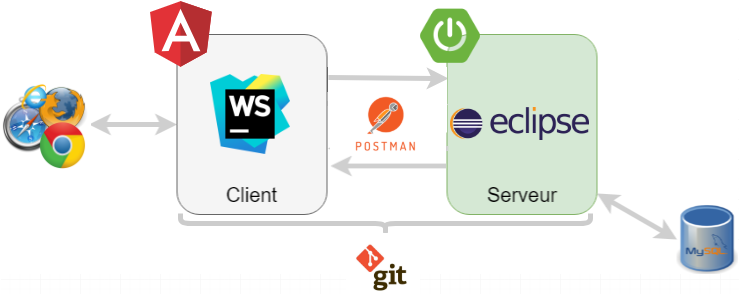
\includegraphics[width=1\textwidth]{chapitre5/Figures/outils.png}
  \caption{Outils utilisés}
\end{figure}

La liste non exhaustive suivante donne une idée sur notre environnement de travail :
\begin{itemize}[label=\textbullet]
  \item Astah permettant la modélisation UML
  \item Eclipse est l'IDE utilisé pour développer le Back-end
  \item Git est le logiciel consacré à la gestion du code source
  \item MySQL a pour but la sauvegarde et la restitution des données
  \item Postman est l'outil choisi pour tester les API REST
  \item WebStorm est l'IDE utilisé pour développer le Front-end
\end{itemize}

Les outils susmentionnés sont décrits en détails dans l'Annexe C.
\section{Réalisation}
L’objectif de cette partie est de donner un aperçu sur les différentes interfaces (IHMs) du système développé, ainsi que les fonctionnalités offertes à l’utilisateur.

\begin{itemize}[label=\textbullet]
%authentification
\item \textbf{Authentification}
Pour accéder aux différentes fonctionnalités de la plateforme, l’utilisateur doit s’authentifier (Figure 5.2)
\begin{figure}[h!]  
 \centering
    
\includegraphics[width=1\textwidth]{chapitre5/Figures/cnx.png}
  \caption{Page d’authentification}
\end{figure}

\begin{itemize}
\item Si les informations entrées par l’utilisateur ne sont pas valides, un message d’avertissement s’affiche (Figure 5.3)
\end{itemize}
\newpage
\begin{figure}[h!]  
 \centering
    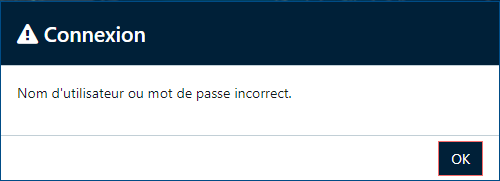
\includegraphics[width=0.7\textwidth]{chapitre5/Figures/errorcnx.png}
  \caption{Message d'avertissement}
\end{figure}

\begin{itemize}
\item Si l’utilisateur oublie son mot de passe, un mail sera envoyé à sa boîte mail (Figure 5.4)
\end{itemize}
\begin{figure}[h!]  
 \centering
    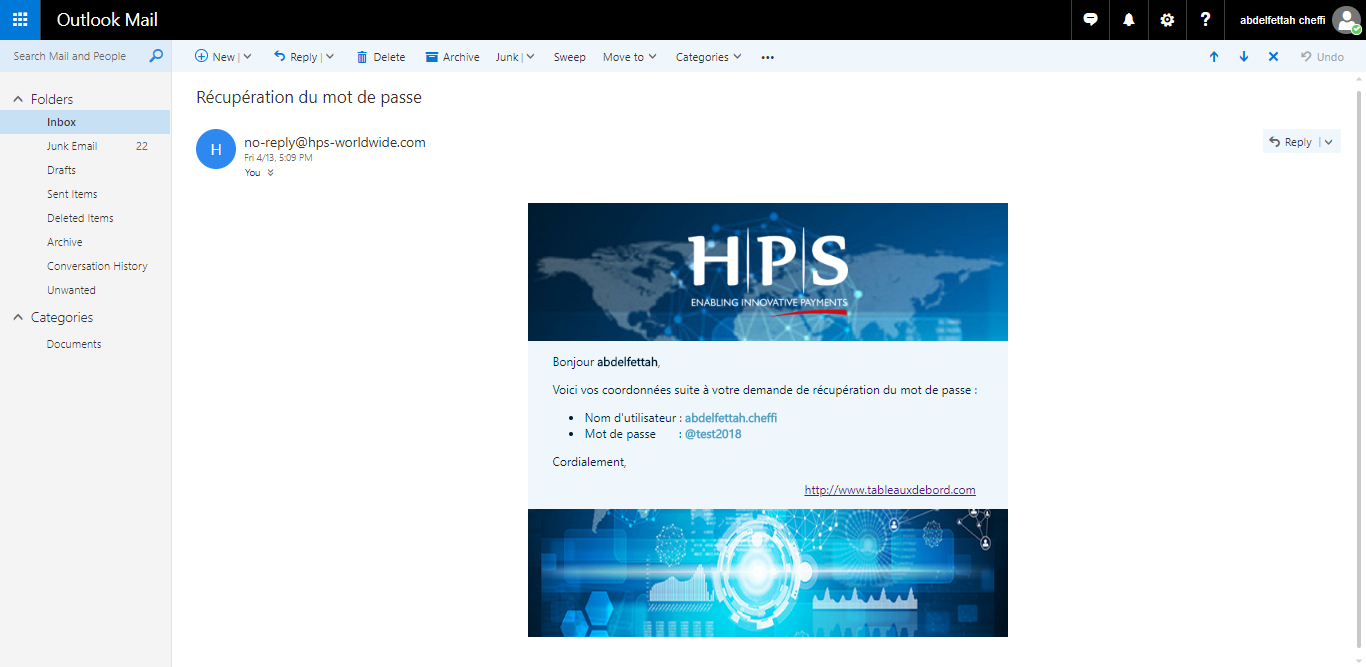
\includegraphics[width=1\textwidth]{chapitre5/Figures/mdpoublie.png}
  \caption{Mail de récupération du mot de passe}
\end{figure}

\begin{itemize}
\item Si la connexion est réussite alors l’utilisateur sera redirigé vers la page d’accueil (Figure 5.5) où il pourra consulter l’application selon son rôle et les droits d’accès qui lui sont attribués 
\end{itemize}
\newpage
\begin{figure}[h!]  
 \centering
    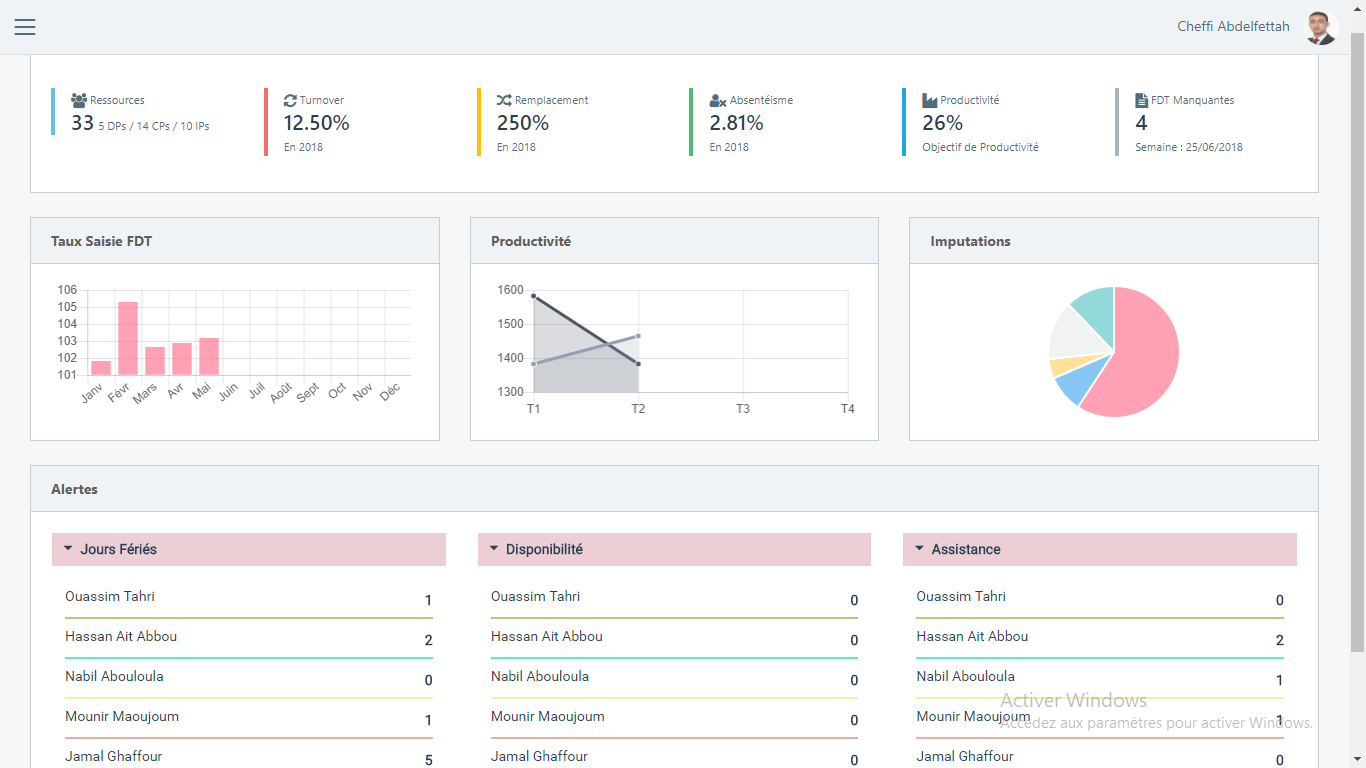
\includegraphics[width=1\textwidth]{chapitre5/Figures/acceuil.png}
  \caption{Page d'accueil}
\end{figure}

\end{itemize}

Cette interface est composée des widgets généraux (nombre ressources, remplacement, absentéisme, FDT manquantes, ...), des graphes (Taux de sasie des FDT, productivité, imputations) ainsi que des alertes.\\
%parametrage
\begin{itemize}[label=\textbullet]
	\item \textbf{Module de paramétrage}
	Ce module permet à l'utilisateur (administrateur et sous-administrateur) de définir les paramètres de l’application.

	\begin{itemize}[label=\textbullet]
	\item Partie administration : cette partie offre les fonctionnalités d'ajout, modification, recherche et suppression et se compose de 4 volets généraux:
	\begin{itemize}
	\item Gestion des agences 
      	\item Gestion des utilisateurs 
     	 \item Gestion des profils 
      	\item Gestion des compétences 
	\end{itemize}
	\end{itemize}
	\newpage
%gestion agence
	\subsubsection*{Exemple "gestion des agences" : }
	\begin{itemize}
			\item Ajouter agence :  l'utilisateur doit respecter la validation correcte des champs des formulaires.
			\begin{figure}[h!]  
			\centering
			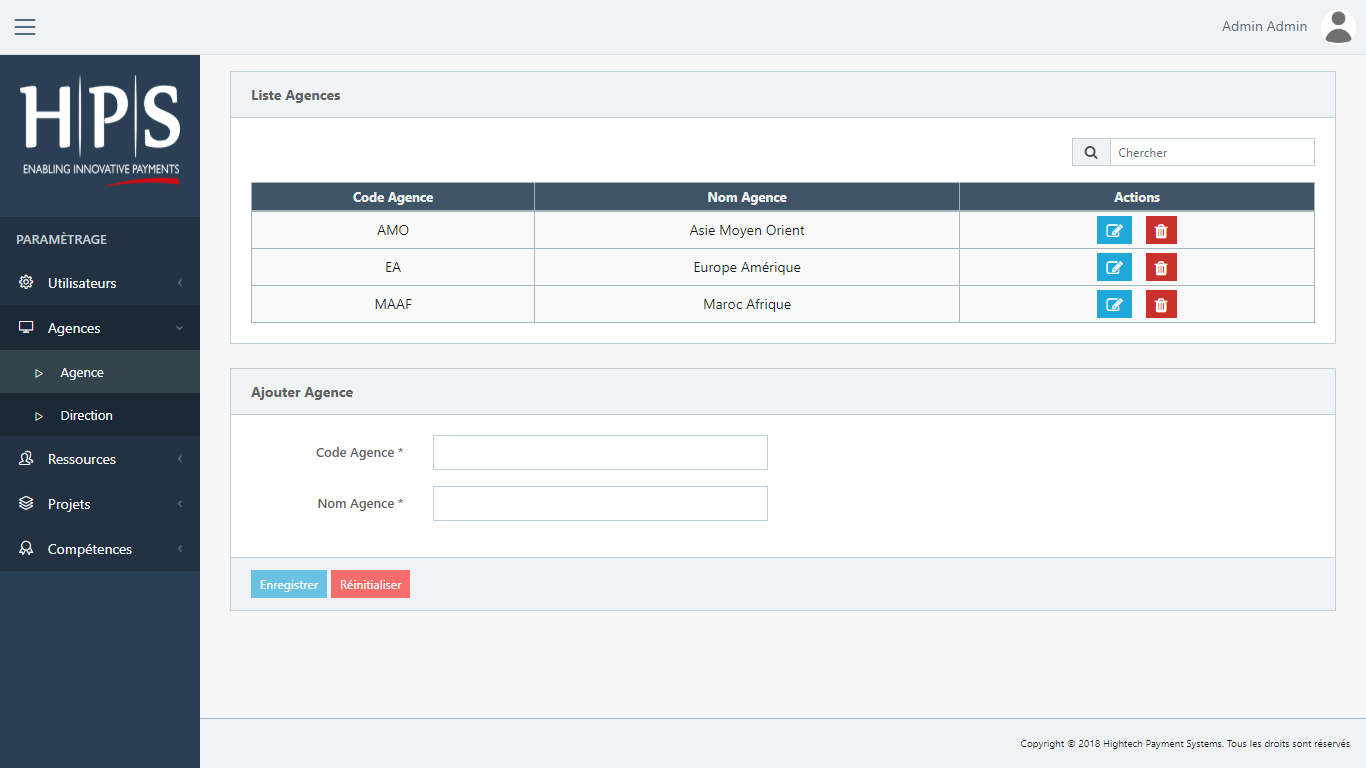
\includegraphics[width=0.9\textwidth]{chapitre5/Figures/addagence.png}
			\caption{Ajouter agence}
			\end{figure}
			\item Supprimer agence : l'utilisateur peut supprimer une agence en cliquant sur le bouton rouge qui correspond à l'enregistrement à supprimer. Un message de confirmation sera affiché
			\begin{figure}[h!]  
			\centering
			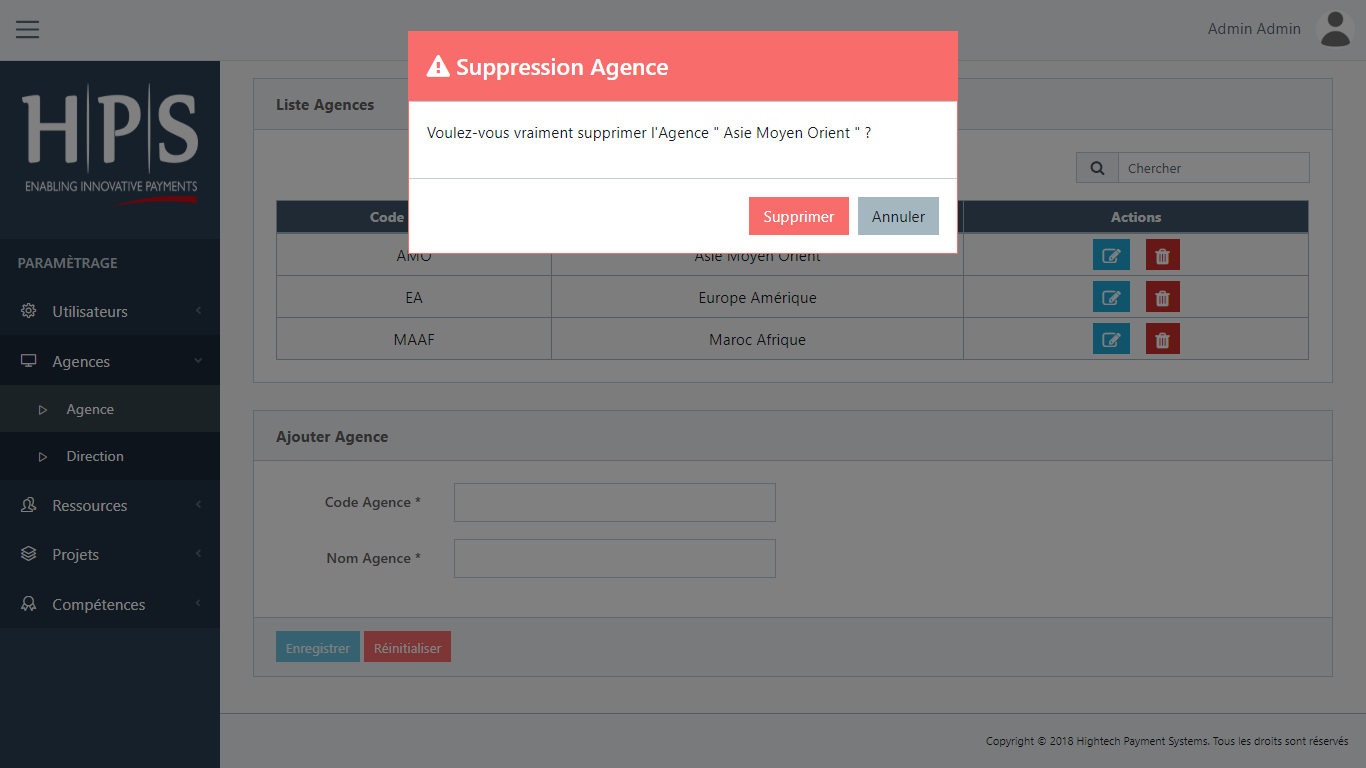
\includegraphics[width=0.9\textwidth]{chapitre5/Figures/supagence.png}
			\caption{Supprimer agence}
			\end{figure}
\newpage
			\item Modifier agence : l'utilisateur choisit un enregistrement à modifier, en cliquant dessus il sera redirigé à l'interface suivante
			\begin{figure}[h!]  
			\centering
			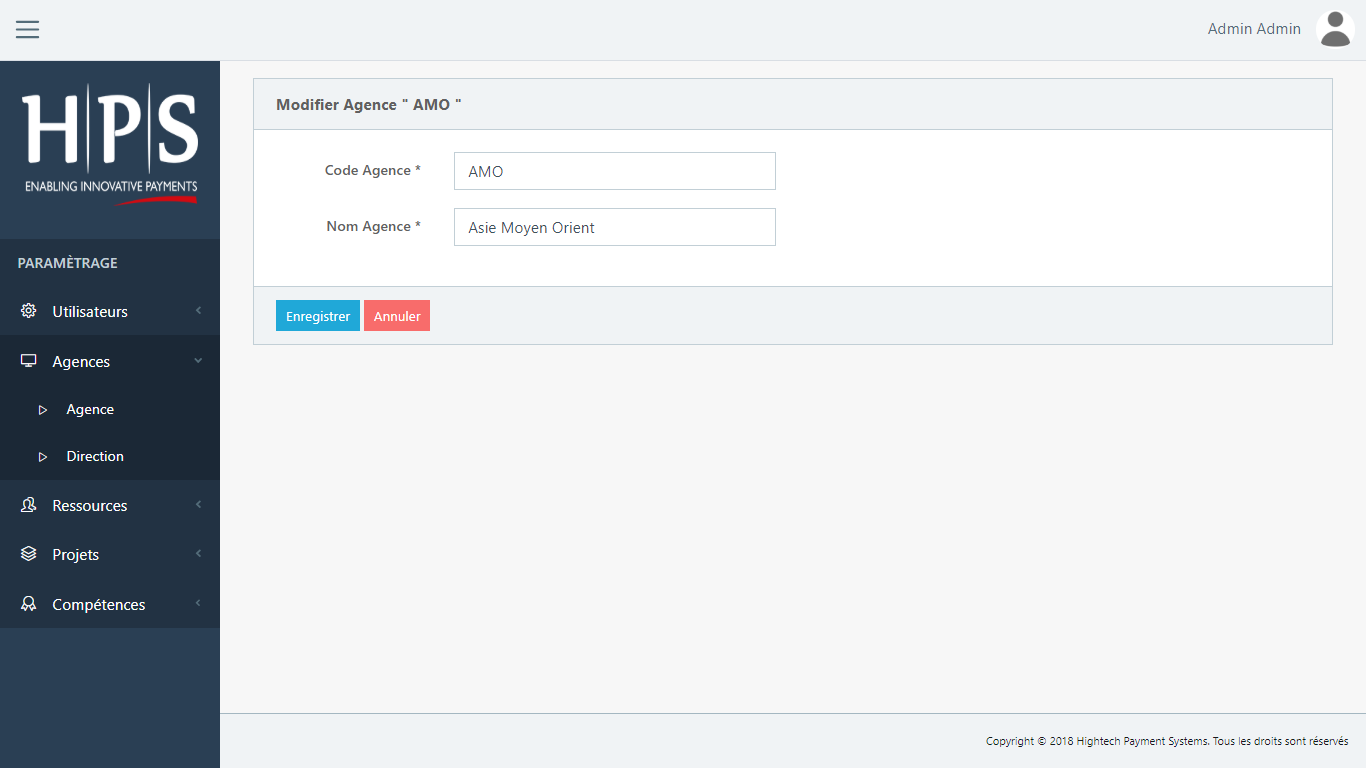
\includegraphics[width=1\textwidth]{chapitre5/Figures/modagence.png}
			\caption{Modifier agence}
			\end{figure}
			\end{itemize}

\begin{itemize}[label=\textbullet]
		\item Partie sous-administration : cette partie offre les fonctionnalités d’ajout, modification, recherche et suppression et se compose de 4 volets relatifs à l'agence de l'utilisateur connecté :
		\begin{itemize}
		\item Gestion des clients
      		\item Gestion des ressources
      		\item Gestion des pays et régions
      		\item Gestion des droits d'accès
		\end{itemize}
	\end{itemize}

%gestion ressource
\subsubsection*{Exemple "gestion des ressources" : }
\begin{itemize}
			\item Ajouter ressource projet :  l'utilisateur doit respecter la validation correcte des champs des formulaires.  \newpage
			\begin{figure}[h!]  
			\centering
			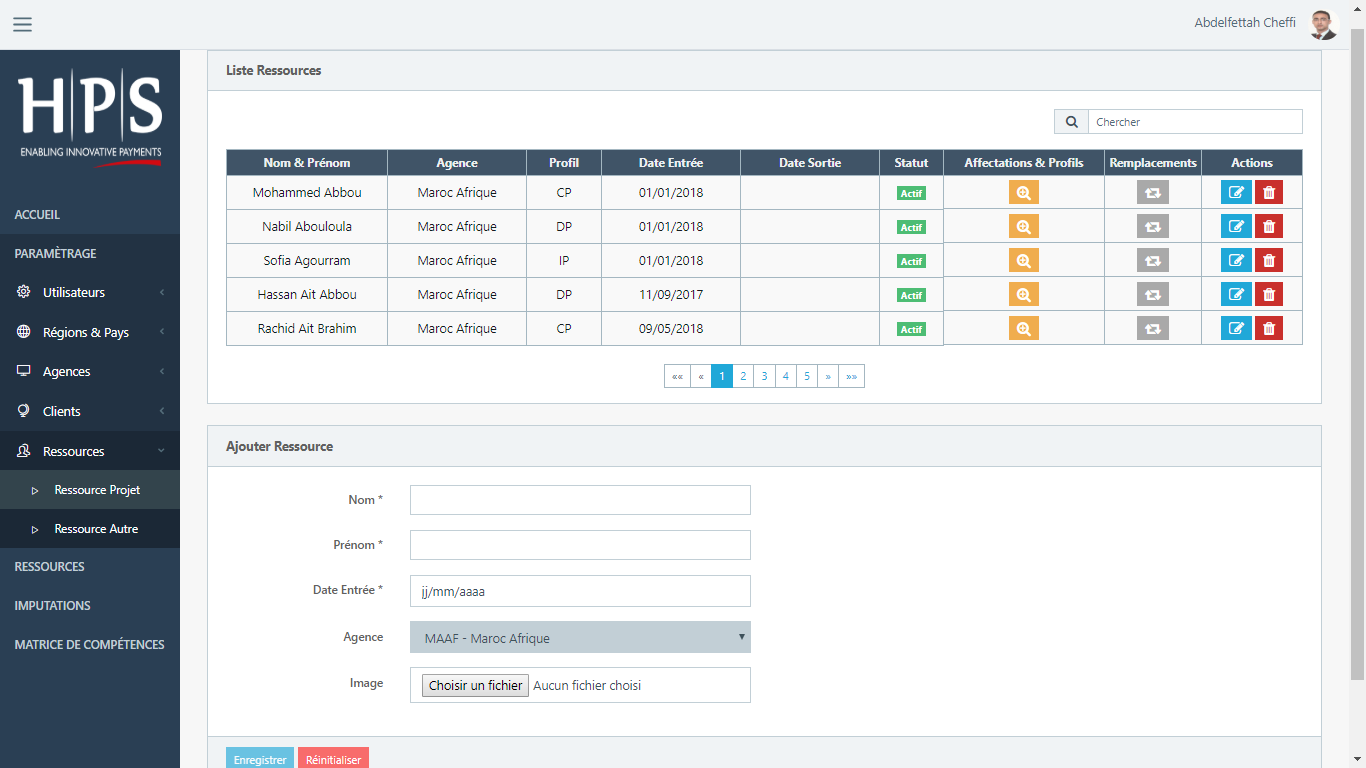
\includegraphics[width=1\textwidth]{chapitre5/Figures/addressource.png}
			\caption{Ajouter ressource projet}
			\end{figure}
			\item Supprimer ressouce projet : l'utilisateur peut supprimer une ressource projet en cliquant sur le bouton rouge qui correspond à l'enregistrement à supprimer. Un message de confirmation sera affiché
			\begin{figure}[h!]  
			\centering
			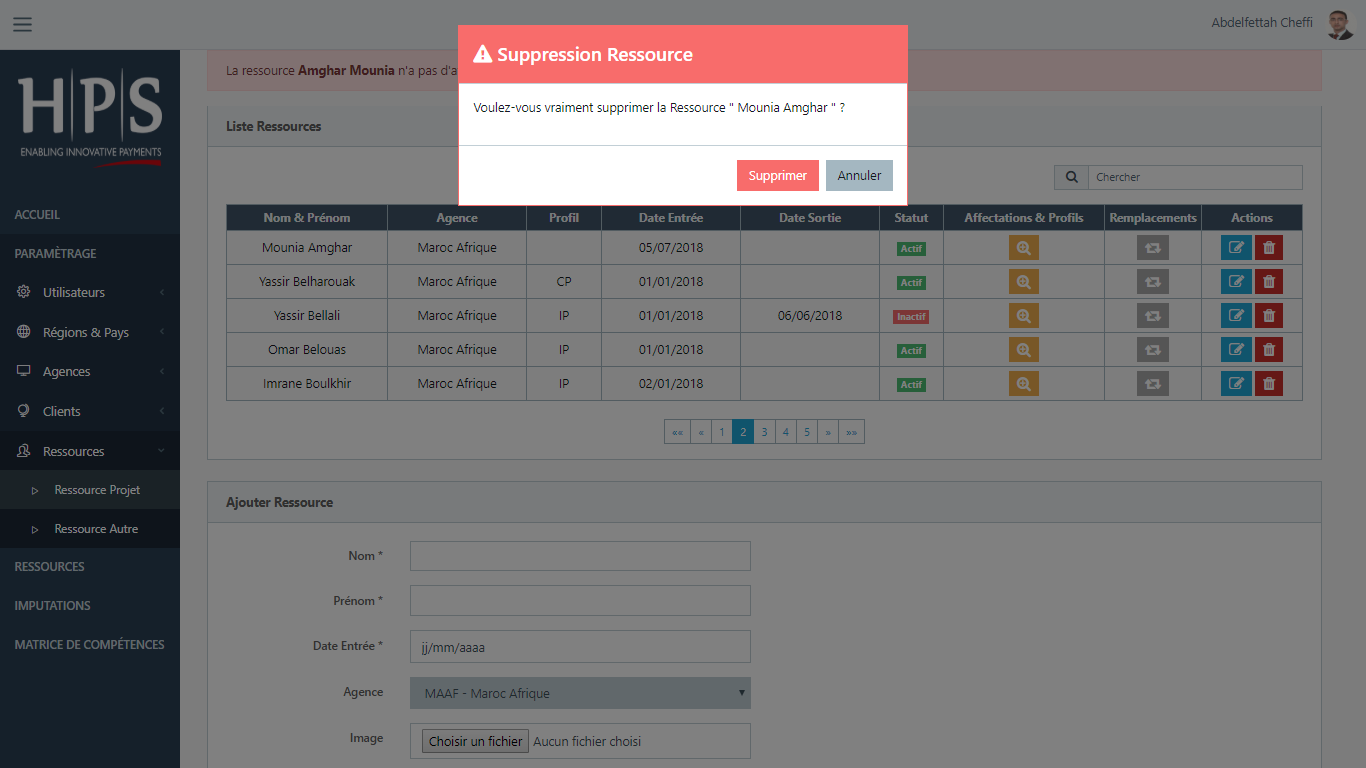
\includegraphics[width=1\textwidth]{chapitre5/Figures/supressource.png}
			\caption{Supprimer ressource projet}
			\end{figure}
			\item Modifier ressouce projet : l'utilisateur choisit un enregistrement à modifier, en cliquant dessus il sera redirigé à l'interface suivante
			\begin{figure}[h!]  
			\centering
			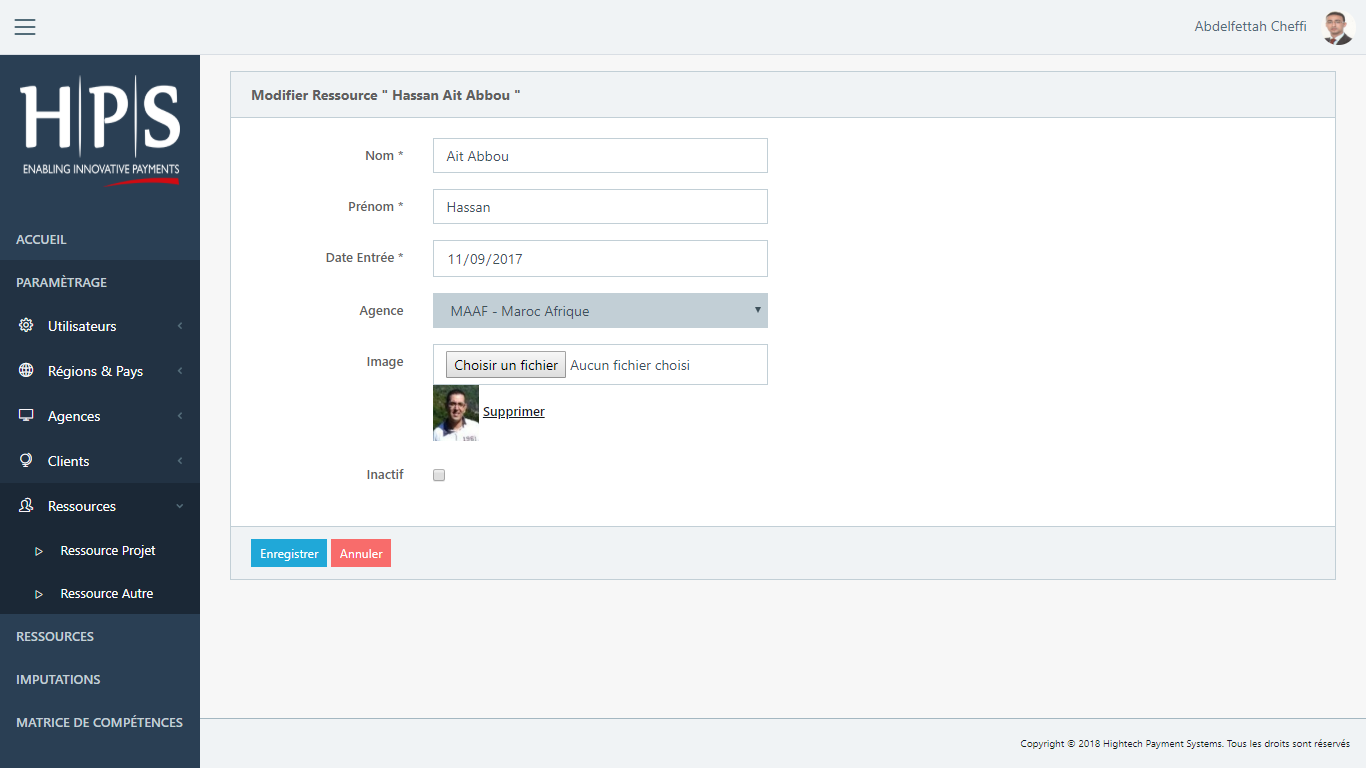
\includegraphics[width=1\textwidth]{chapitre5/Figures/modressource.png}
			\caption{Modifier ressource projet}
			\end{figure}
			\item Remplacer ressource projet : l'utilisateur choisit une ressource à remplacer, en cliquant sur le bouton correspondant il sera redirigé à l'interface suivante où il pourra choisir la ressource qui va la remplacer
			\begin{figure}[h!]  
			\centering
			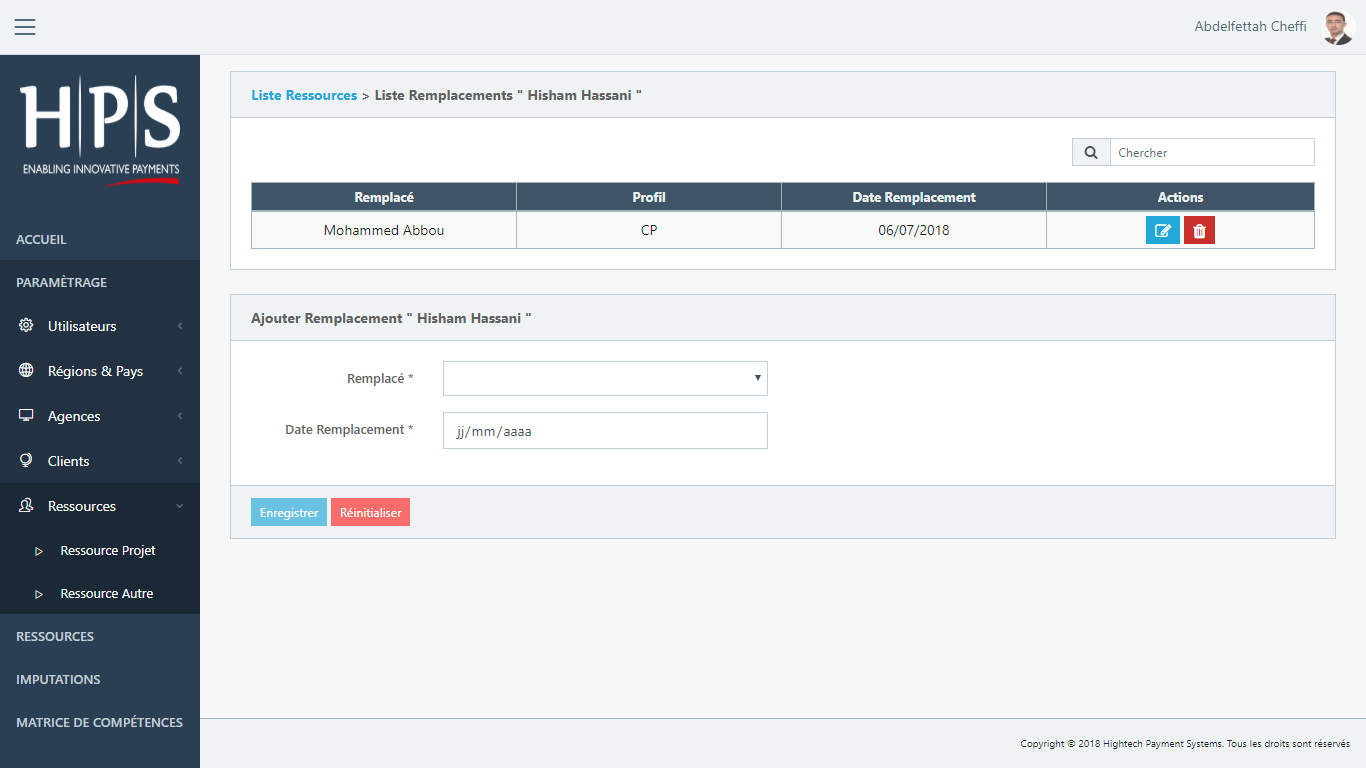
\includegraphics[width=1\textwidth]{chapitre5/Figures/rempressource.png}
			\caption{Remplacer ressource projet}
			\end{figure}
			\item Affecter ressource projet : quand une ressource est ajoutée, elle n'as pas de profil, par suite il faut ajouter une affectation à la ressource. Une affectation pourra être ajouter, modifier ou supprimer
			\begin{figure}[h!]  
			\centering
			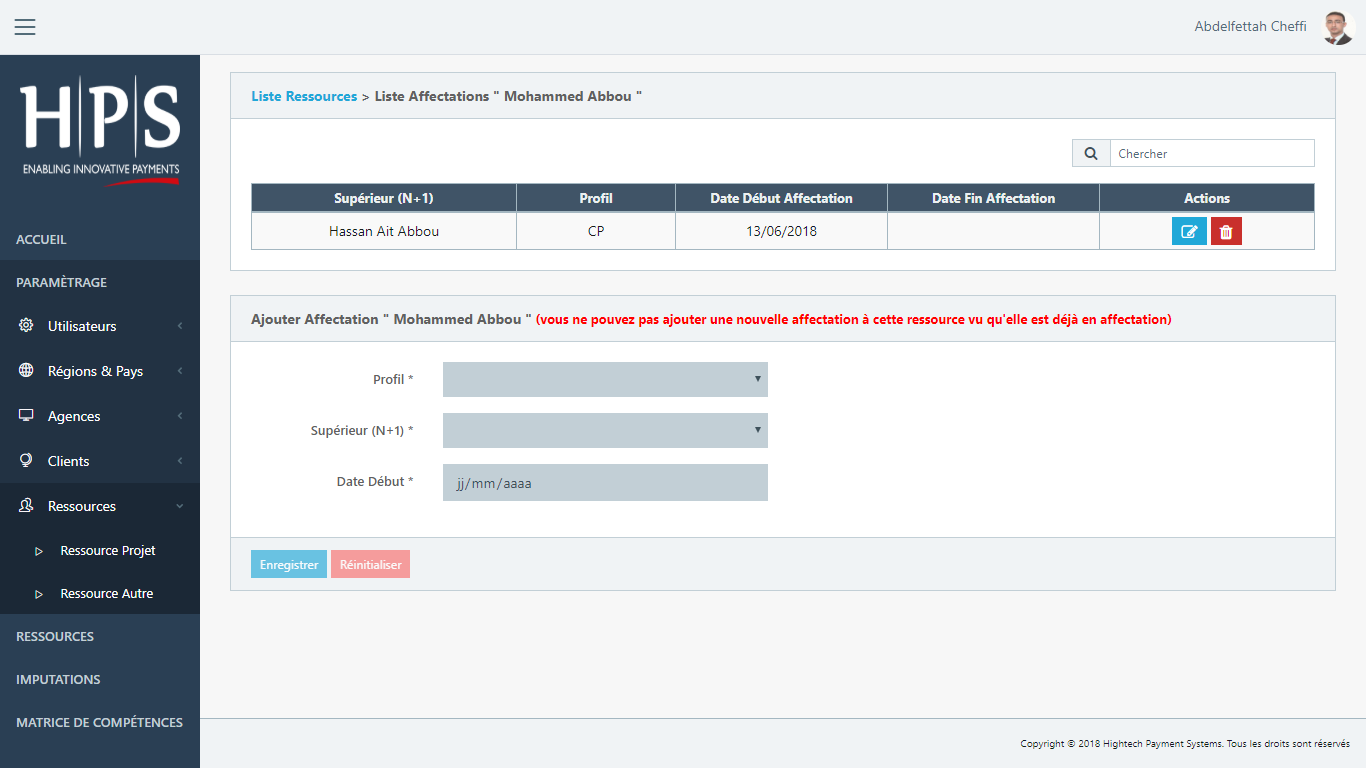
\includegraphics[width=1\textwidth]{chapitre5/Figures/affressource.png}
			\caption{Affecter ressource projet}
			\end{figure}
			\end{itemize}
%gestion des droit d'accées
\subsubsection*{Exemple "gestion des droits d'accès" : }
Cette interface permet au sous-administrateur d'attribuer les droits d'accès d'une rubrique à un profil
\begin{figure}[h!]  
			\centering
			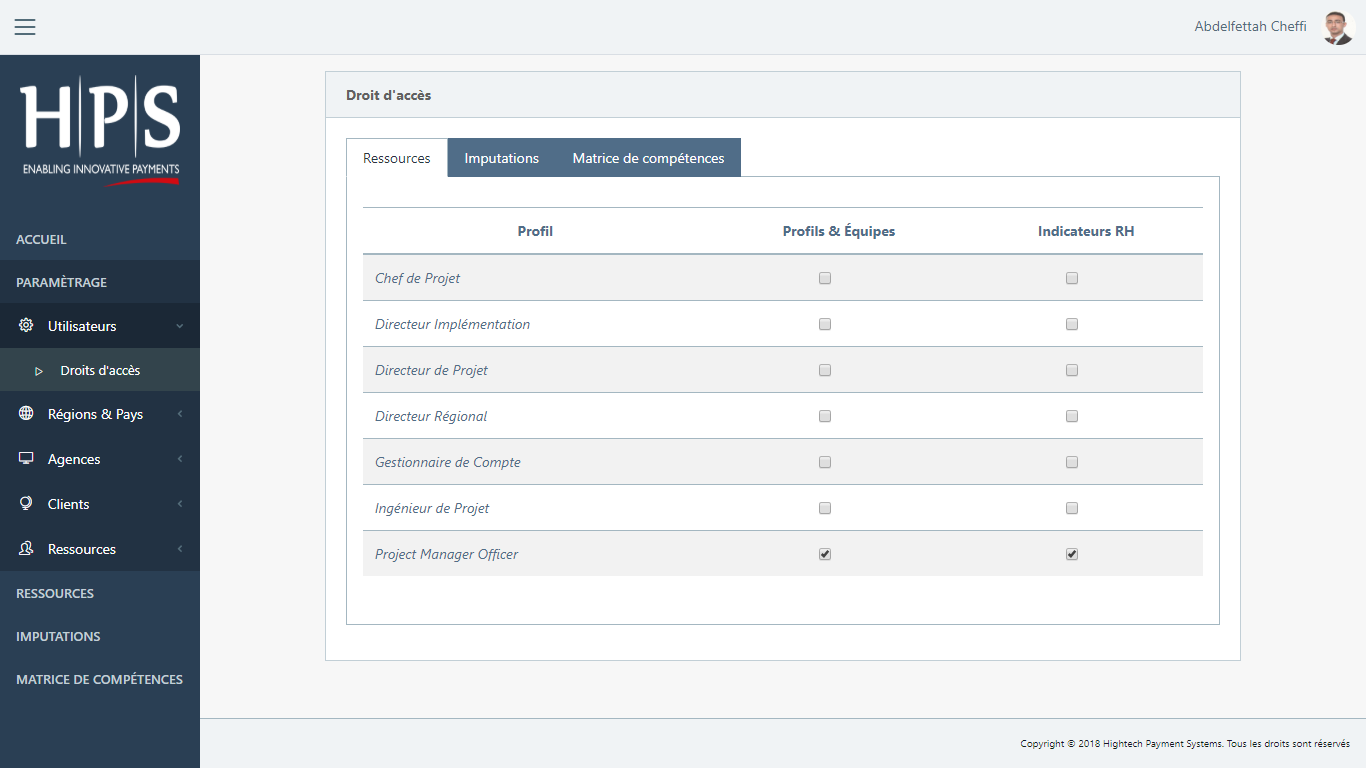
\includegraphics[width=1\textwidth]{chapitre5/Figures/droit.png}
			\caption{Droits d'accès}
			\end{figure}


%%%%module resspources
\item \textbf{Module de suivi des ressources}
	Ce module permet aux collaborateurs le suivi des resssources.
\begin{itemize}
\item \textbf{Profils et équipes }
\begin{figure}[h!]  
			\centering
			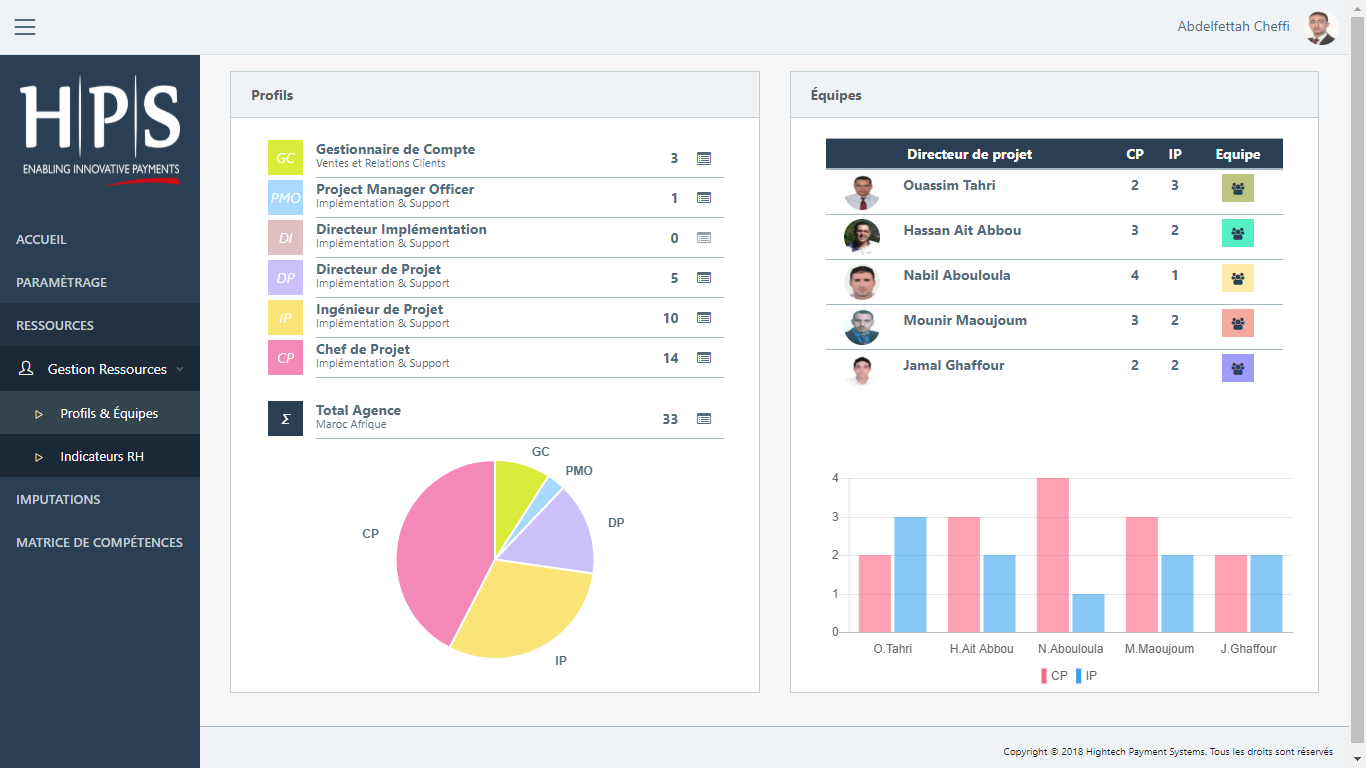
\includegraphics[width=1\textwidth]{chapitre5/Figures/proequ.png}
			\caption{Profils et équipes}
			\end{figure}
\\
Cette interface permet à l'utilisateur de consulter le nombre de ressources et leurs noms par profil (Figure 5.16) ainsi que les équipes de chaque directeur de projet (Figure 5.17).
\begin{figure}[h]
    \begin{minipage}[c]{.46\linewidth}
        \centering
        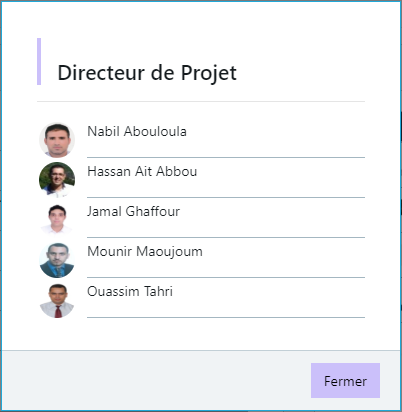
\includegraphics[width=1\textwidth]{chapitre5/Figures/profil.png}
        \caption{Ressources par profil}
    \end{minipage}
    \hfill%
    \begin{minipage}[c]{.46\linewidth}
        \centering
        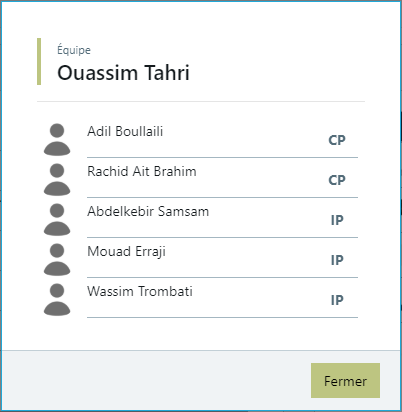
\includegraphics[width=1\textwidth]{chapitre5/Figures/equipes.png}
        \caption{Equipes par DP}
    \end{minipage}
\end{figure}
\newpage
\item \textbf{Indicateurs RH }
\begin{figure}[h!]  
			\centering
			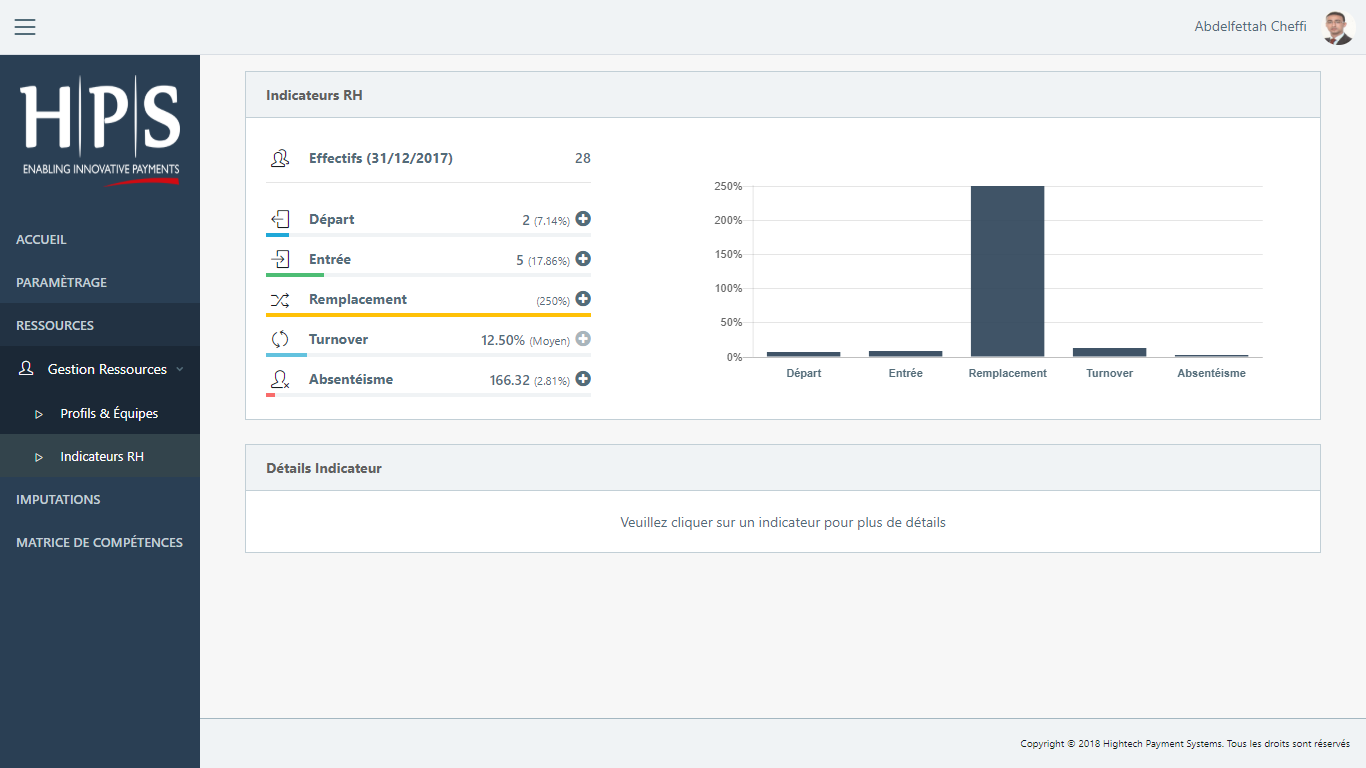
\includegraphics[width=1\textwidth]{chapitre5/Figures/indicateur.png}
			\caption{Indicateurs RH}
			\end{figure}
\\
  Cette interface représente le nombre des départs et d'entrées ainsi que le taux de remplacement, turnover et absentéisme dans l'agence.\\
Pour chaque indicateur, on peut avoir les détails (Figure 5.19)
\begin{figure}[h!]  
			\centering
			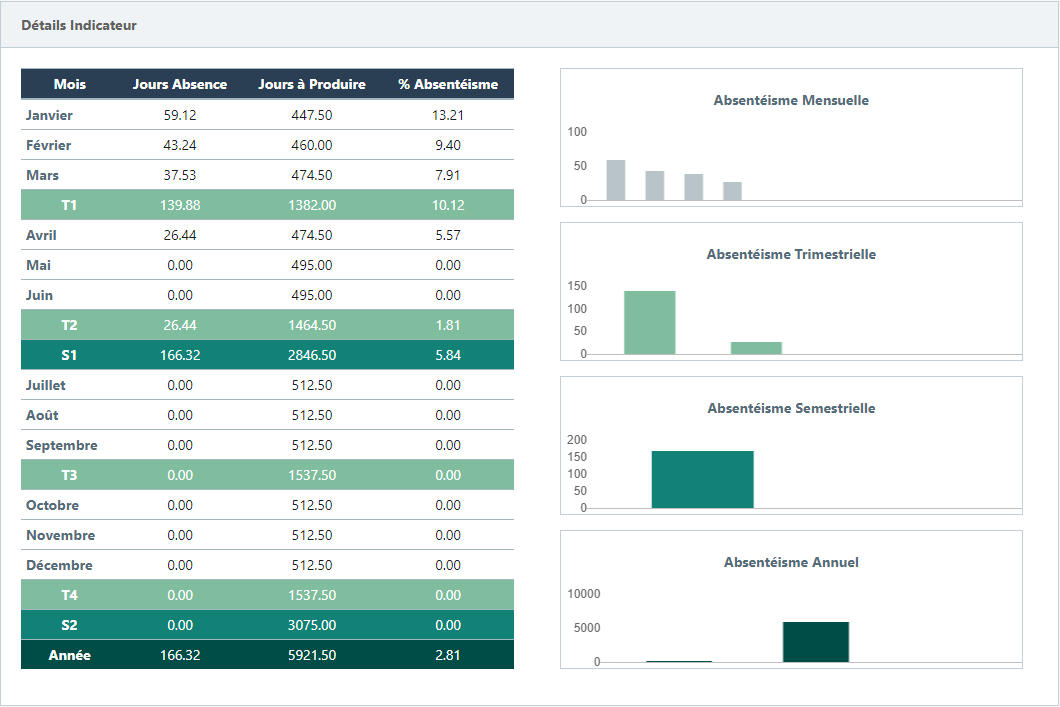
\includegraphics[width=0.8\textwidth]{chapitre5/Figures/details.png}
			\caption{Détails de l'indicateur absentéisme}
			\end{figure}
\end{itemize}
%%%suivi imputation
\item \textbf{Module de suivi des imputations}
	Ce module permet aux collaborateurs de représenter les statistiques liées à la saisie des feuilles de temps des ressources.
\begin{itemize}
\item \textbf{Suivi des FDT}
\begin{figure}[h!]  
			\centering
			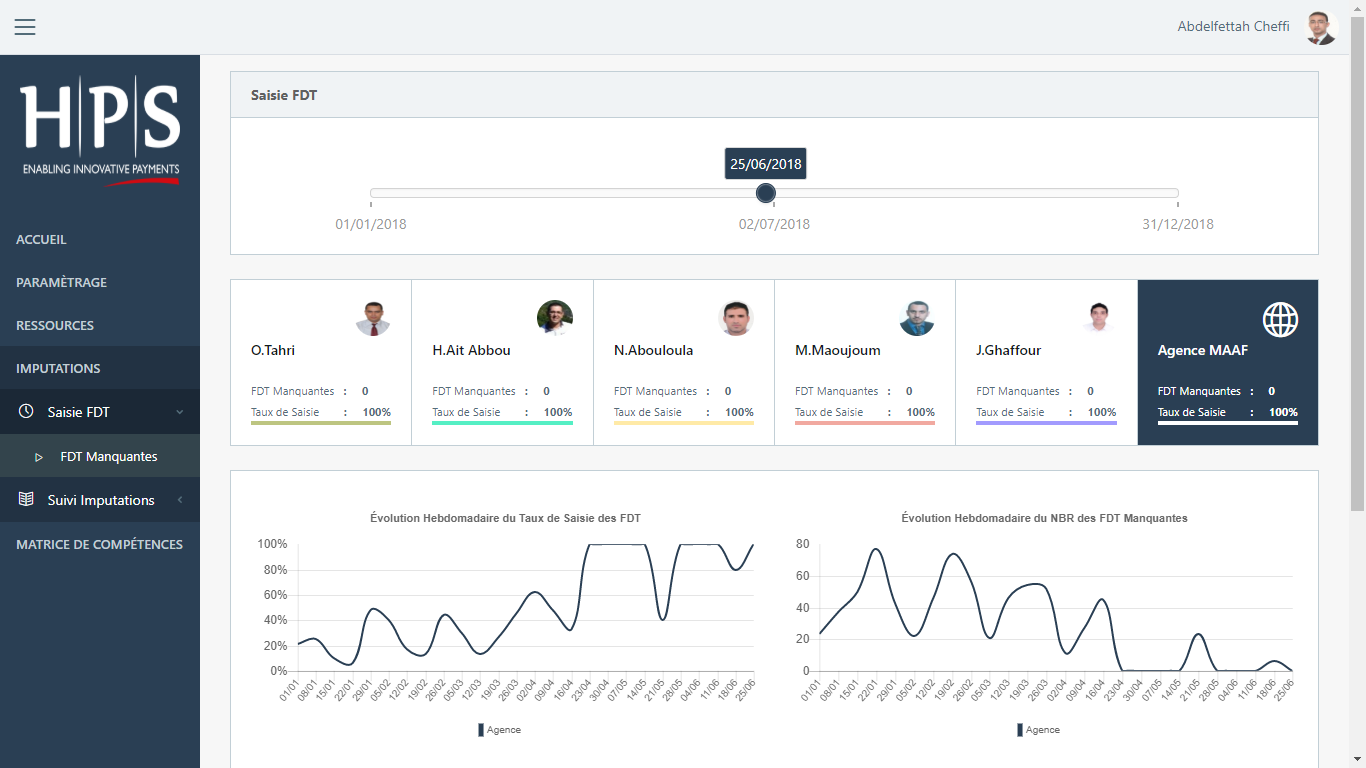
\includegraphics[width=1\textwidth]{chapitre5/Figures/fdt.png}
			\caption{Suivi des FDT}
			\end{figure}
\\
Cette interface se divise en deux parties, la première permet l'affichage des FDT manquantes et le taux de saisie par directeur de projet et par agence pour chaque semaine ainsi que la saisie des FDT manquantes (Figure 5.21). La deuxième affiche l'évolution hebdomadaire du taux de saisie et FDT manquantes par agence et par directeur de projet (Figure 5.22)
\begin{figure}[h]
    \begin{minipage}[c]{.46\linewidth}
        \centering
        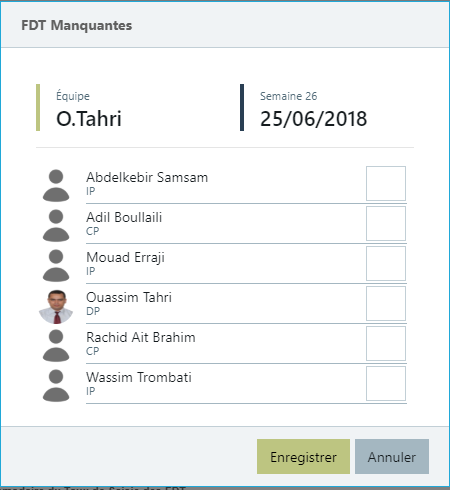
\includegraphics[width=0.97\textwidth]{chapitre5/Figures/saisiefdt.png}
        \caption{Ressources par profil}
    \end{minipage}
    \hfill%
    \begin{minipage}[c]{.46\linewidth}
        \centering
        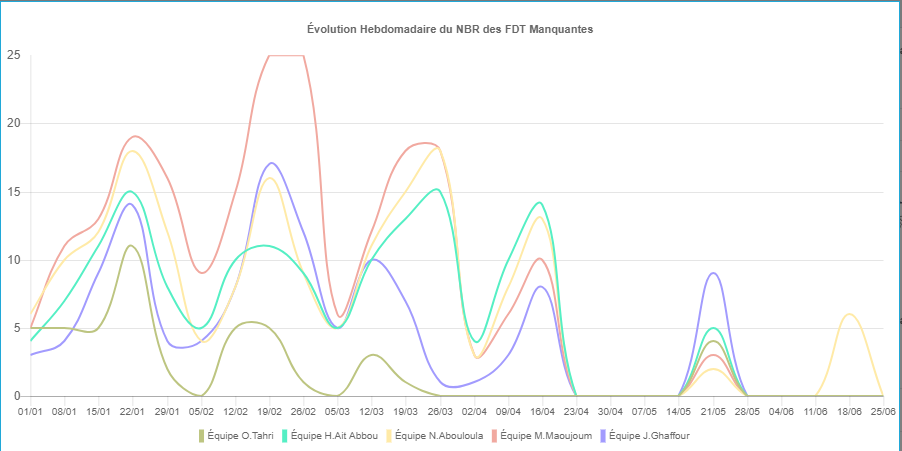
\includegraphics[width=1\textwidth]{chapitre5/Figures/evolution.png}
        \caption{évolution hebdomadaire du taux de saisie par directeur de projet}
    \end{minipage}
\end{figure}
\newpage
\item \textbf{Taux de Saisie}
\begin{figure}[h!]  
			\centering
			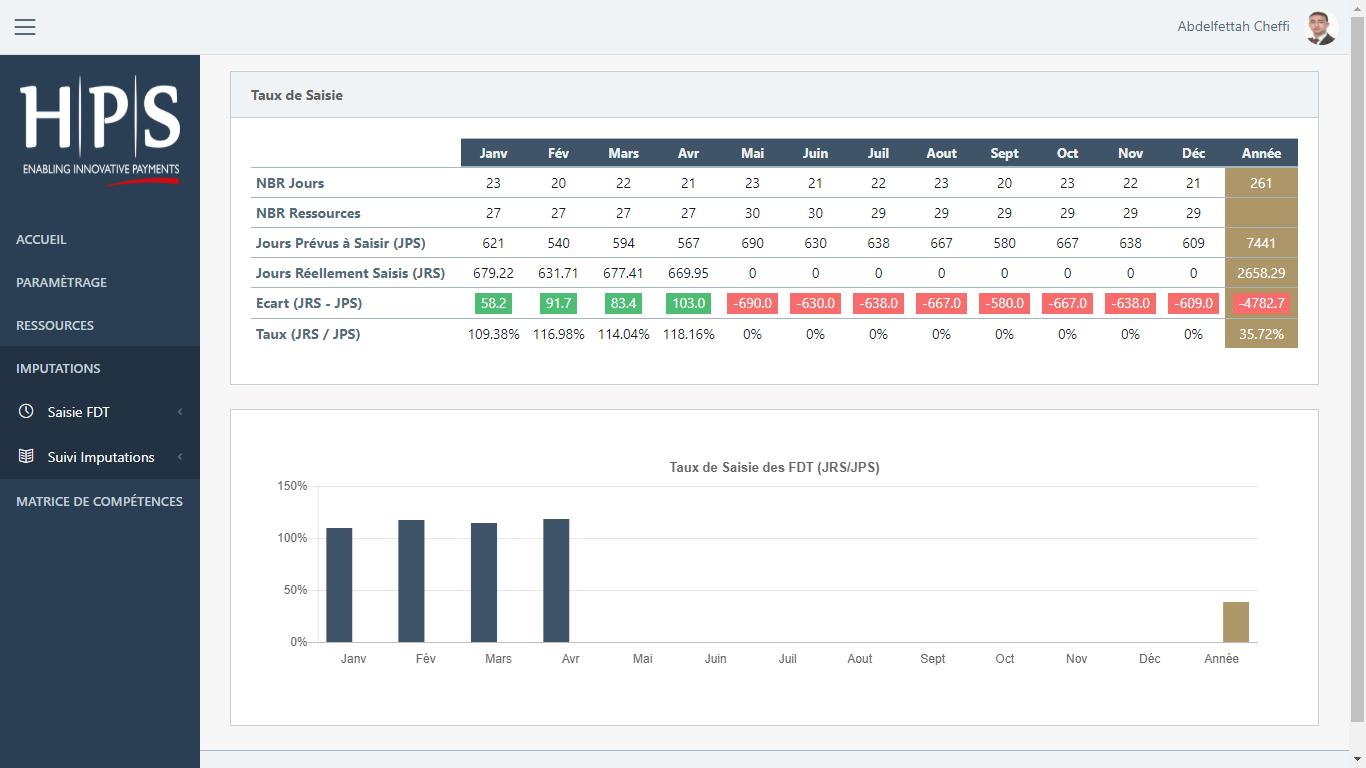
\includegraphics[width=0.92\textwidth]{chapitre5/Figures/taux.png}
			\caption{Taux de Saisie}
			\end{figure}
\\
Cette interface représente le taux de saisie des FDT mensuellement de l'agence.
\end{itemize}
%%matrice des competence
\item \textbf{Module de la matrice de compétences}
Ce module permet d’évaluer les compétences des ressources et de connaitre réellement leurs niveaux sur plusieurs domaines.
\begin{itemize}
\item \textbf{Evaluation}
\begin{figure}[h!]  
			\centering
			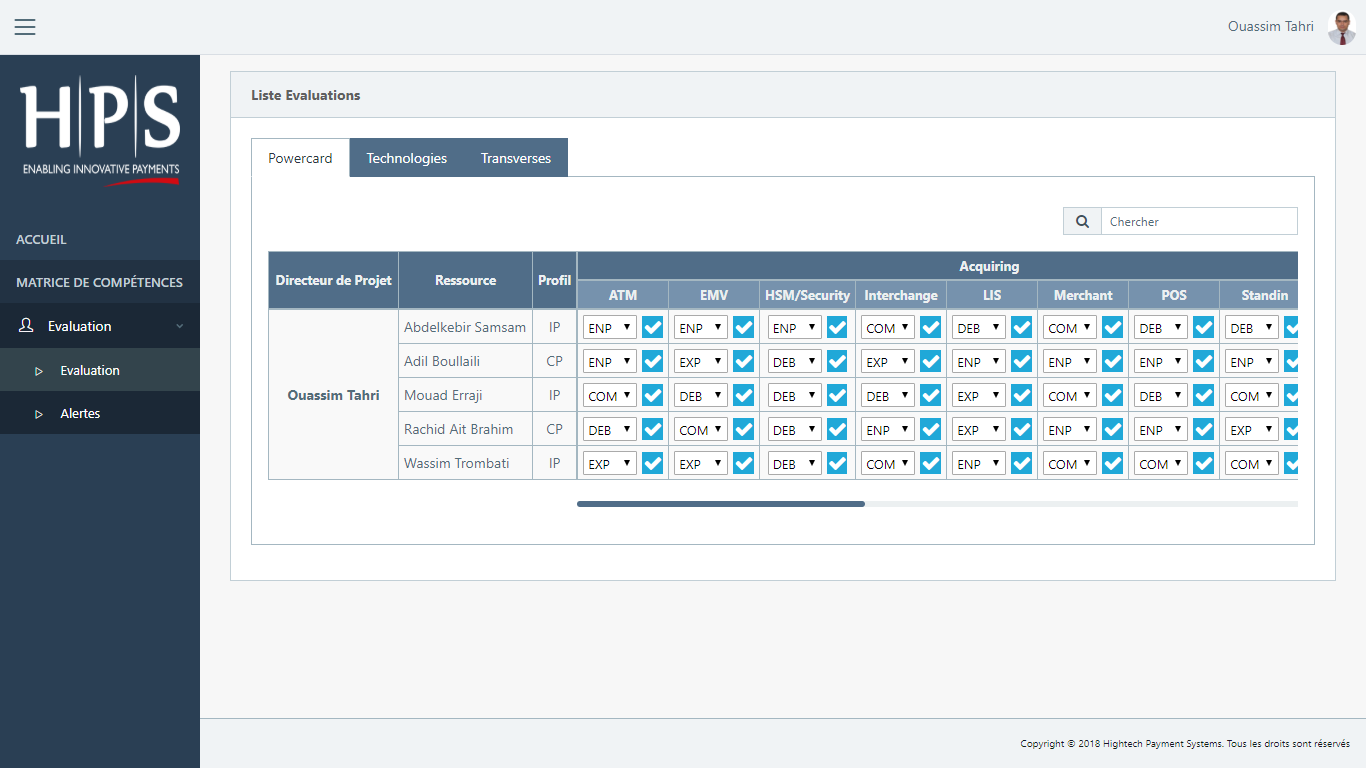
\includegraphics[width=0.92\textwidth]{chapitre5/Figures/evaluation.png}
			\caption{Evaluation}
			\end{figure}
\newpage
Cette interface permet au directeur de projet d'évaluer les compétences de ces ressources.
\item \textbf{Synthèse}
\begin{figure}[h!]  
			\centering
			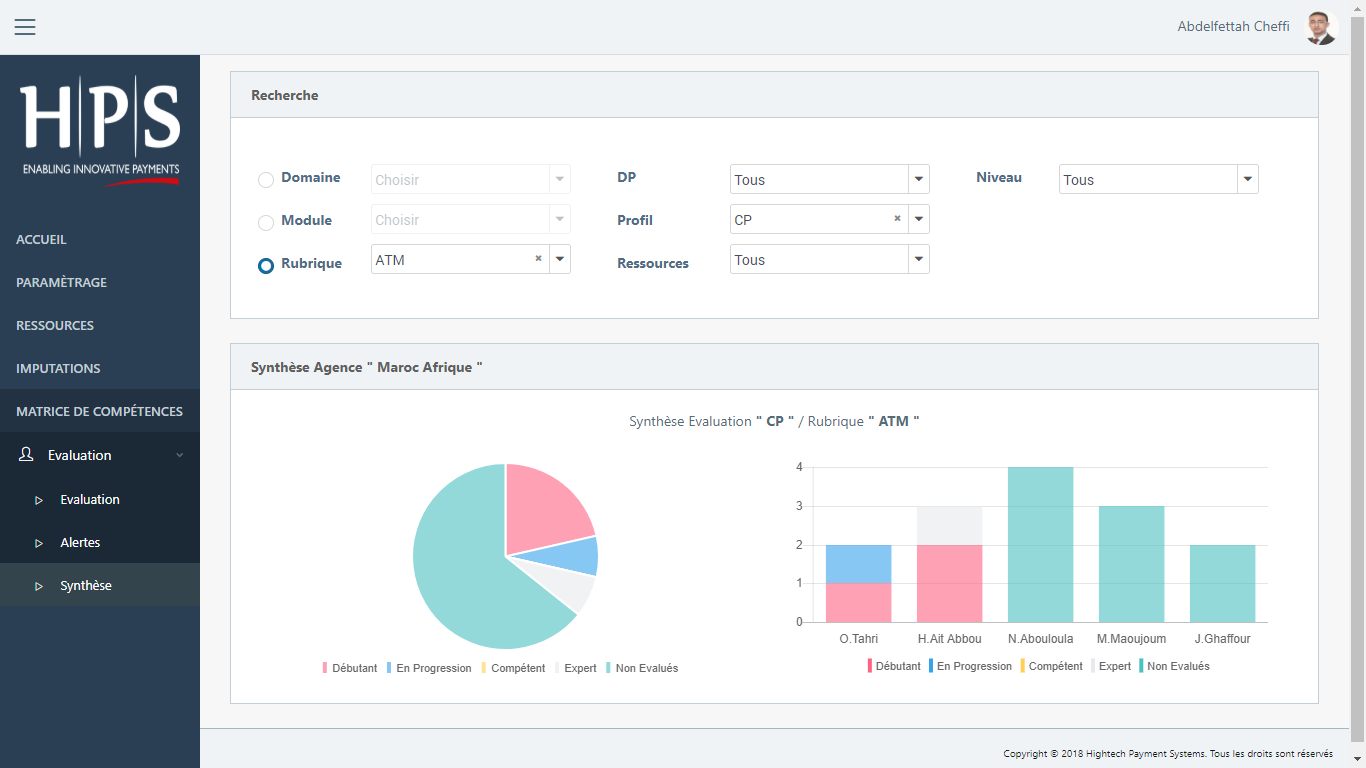
\includegraphics[width=1\textwidth]{chapitre5/Figures/synthese.png}
			\caption{Synthèse}
			\end{figure}
\\
Cette interface permet d'afficher des graphes syntétisant l'évaluation des resources selon des critères définis par l'utilisateur.
\end{itemize}
\end{itemize}
\section{Travail réalisé et reste à faire}
L'ensemble du projet contient 5 modules (paramétrage, suivi des ressources, suivi des imputations, la matrice des compétences et suivi des projets), on a réalisé les modules paramétrage, suivi des ressources, une partie de suivi des imputations ( les FDT) et la matrice des compétences. La partie restante du module suivi des imputations (Productivité) et le module suivi des projets restent à développer.
\newpage
\begin{figure}[h!]  
	\centering
	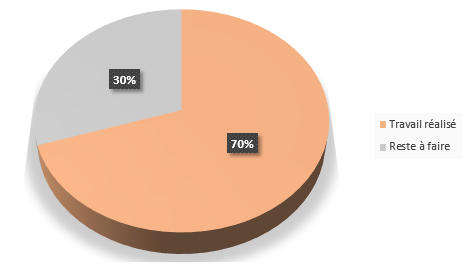
\includegraphics[width=1\textwidth]{chapitre5/Figures/avancement.png}
	\caption{Pourcentage d'avancement par rapport au cahier de charge}
\end{figure}
\section*{Conclusion}
Ce dernier chapitre a servi à introduire les outils de développement utilisés afin de présenter par la suite le travail réalisé pour concrétiser le travail mené dans l’étude fonctionnelle ainsi que le reste à faire.